\documentclass[12pt,letterpaper]{article}
\usepackage{graphicx,textcomp}
\usepackage{natbib}
\usepackage{setspace}
\usepackage{fullpage}
\usepackage{color}
\usepackage[reqno]{amsmath}
\usepackage{amsthm}
\usepackage{fancyvrb}
\usepackage{amssymb,enumerate}
\usepackage[all]{xy}
\usepackage{endnotes}
\usepackage{lscape}
\newtheorem{com}{Comment}
\usepackage{float}
\usepackage{hyperref}
\newtheorem{lem} {Lemma}
\newtheorem{prop}{Proposition}
\newtheorem{thm}{Theorem}
\newtheorem{defn}{Definition}
\newtheorem{cor}{Corollary}
\newtheorem{obs}{Observation}
\usepackage[compact]{titlesec}
\usepackage{dcolumn}
\usepackage{tikz}
\usetikzlibrary{arrows}
\usepackage{multirow}
\usepackage{xcolor}
\newcolumntype{.}{D{.}{.}{-1}}
\newcolumntype{d}[1]{D{.}{.}{#1}}
\definecolor{light-gray}{gray}{0.65}
\usepackage{url}
\usepackage{listings}
\usepackage{color}

\definecolor{codegreen}{rgb}{0,0.6,0}
\definecolor{codegray}{rgb}{0.5,0.5,0.5}
\definecolor{codepurple}{rgb}{0.58,0,0.82}
\definecolor{backcolour}{rgb}{0.95,0.95,0.92}

\lstdefinestyle{mystyle}{
	backgroundcolor=\color{backcolour},   
	commentstyle=\color{codegreen},
	keywordstyle=\color{magenta},
	numberstyle=\tiny\color{codegray},
	stringstyle=\color{codepurple},
	basicstyle=\footnotesize,
	breakatwhitespace=false,         
	breaklines=true,                 
	captionpos=b,                    
	keepspaces=true,                 
	numbers=left,                    
	numbersep=5pt,                  
	showspaces=false,                
	showstringspaces=false,
	showtabs=false,                  
	tabsize=2
}
\lstset{style=mystyle}
\newcommand{\Sref}[1]{Section~\ref{#1}}
\newtheorem{hyp}{Hypothesis}

\title{Problem Set 2}
\date{Due: October 15, 2023}
\author{Applied Stats/Quant Methods 1\\
Zhuo Zhang/Student ID: 23346227}

\begin{document}
	\maketitle
	\section*{Instructions}
\begin{itemize}
	\item Please show your work! You may lose points by simply writing in the answer. If the problem requires you to execute commands in \texttt{R}, please include the code you used to get your answers. Please also include the \texttt{.R} file that contains your code. If you are not sure if work needs to be shown for a particular problem, please ask.
	\item Your homework should be submitted electronically on GitHub.
	\item This problem set is due before 23:59 on Sunday October 15, 2023. No late assignments will be accepted.

\end{itemize}

	
	\vspace{.5cm}
	\section*{Question 1: Political Science}
		\vspace{.25cm}
	The following table was created using the data from a study run in a major Latin American city.\footnote{Fried, Lagunes, and Venkataramani (2010). ``Corruption and Inequality at the Crossroad: A Multimethod Study of Bribery and Discrimination in Latin America. \textit{Latin American Research Review}. 45 (1): 76-97.} As part of the experimental treatment in the study, one employee of the research team was chosen to make illegal left turns across traffic to draw the attention of the police officers on shift. Two employee drivers were upper class, two were lower class drivers, and the identity of the driver was randomly assigned per encounter. The researchers were interested in whether officers were more or less likely to solicit a bribe from drivers depending on their class (officers use phrases like, ``We can solve this the easy way'' to draw a bribe). The table below shows the resulting data.

\newpage
\begin{table}[h!]
	\centering
	\begin{tabular}{l | c c c }
		& Not Stopped & Bribe requested & Stopped/given warning \\
		\\[-1.8ex] 
		\hline \\[-1.8ex]
		Upper class & 14 & 6 & 7 \\
		Lower class & 7 & 7 & 1 \\
		\hline
	\end{tabular}
\end{table}

\begin{enumerate}
	
	\item [(a)]
	Calculate the $\chi^2$ test statistic by hand/manually (even better if you can do "by hand" in \texttt{R}).\\
			\lstinputlisting[language=R, firstline=3, lastline=26]{PS02_zhuo_zhang.R} 
			 \textbf{Result}:\\
			Chi-Squared Test Statistic:  3.79116\\
			
	\vspace{7cm}
	\item [(b)]
	Now calculate the p-value from the test statistic you just created (in \texttt{R}).\footnote{Remember frequency should be $>$ 5 for all cells, but let's calculate the p-value here anyway.}  What do you conclude if $\alpha = 0.1$?\\
		\lstinputlisting[language=R, firstline=30, lastline=48]{PS02_zhuo_zhang.R} 
		 \textbf{Result}:\\
		 Fail to reject the null hypothesis. There is no strong evidence of an association between variables.
	\newpage
	\item [(c)] Calculate the standardized residuals for each cell and put them in the table below.
	\vspace{1cm}
	
	\begin{table}[h]
		\centering
		\begin{tabular}{l | c c c }
			& Not Stopped & Bribe requested & Stopped/given warning \\
			\\[-1.8ex] 
			\hline \\[-1.8ex]
			Upper class  &  &  &  \\
			\\
			Lower class &  &   &   \\
			
		\end{tabular}
	\end{table}
		\lstinputlisting[language=R, firstline=52, lastline=66]{PS02_zhuo_zhang.R} 
		\begin{table}[h]
			\centering
			\begin{center}
			\textbf{{\large result}}
			\end{center}
			\begin{tabular}{l | c c c }
				& Not Stopped & Bribe requested & Stopped/given warning \\
				\\[-1.8ex] 
				\hline \\[-1.8ex]
				Upper class & 0.14 & -0.82 & 0.82 \\
				\\
				Lower class & -0.18 & 1.09  & -1.10  \\
				
			\end{tabular}
		\end{table}
	
	\vspace{7cm}
	\newpage
	\item [(d)] How might the standardized residuals help you interpret the results?  
	\begin{itemize}
		\item Looking at the cell where ``Upper class'' individuals are ``Not Stopped,'' the standardized residual is 0.14.  Since it is close to zero, it suggests that the observed and expected frequencies for this cell are reasonably close, and there may not be a strong association between being in the upper class and not getting stopped.
		\item For the ``Upper class'' group and ``Bribe requested'' cell, the standardized residual is -0.82. This negative value signals that the observed frequency of upper-class individuals requesting a bribe is lower than what would be expected. It suggests that being in the upper class might be associated with a lower likelihood of requesting a bribe.
		\item For the cell corresponding to “Upper class” and “Stopped/given warning,” the standardized residual is 0.82, a positive value.This suggests that the observed frequency of upper-class individuals being stopped or given a warning is higher than expected. It implies that being in the upper class might be associated with a higher likelihood of being stopped or given a warning.
		\item For the cell corresponding to “Lower class” and “Not Stopped,” the standardized residual is -0.18, which is close to zero. It indicates that there may not be a strong association between being in the lower class and not getting stopped.
		\item For the cell corresponding to “Lower class” and “Bribe requested,” the standardized residual is 1.09, indicating that the observed frequency of lower-class individuals requesting a bribe is higher than expected. It suggests that being in the lower class might be associated with a higher likelihood of requesting a bribe.
		\item For the ``Lower class'' group and ``Stopped/given warning,'' the standardized residual is -1.10, a negative value. It suggests that the observed frequency of lower-class individuals being stopped or given a warning is lower than expected. This implies that being in the lower class might be associated with a lower likelihood of experiencing these interactions.
		
		
		
		
		
	\end{itemize}
\end{enumerate}
\newpage

\section*{Question 2: Economics}
Chattopadhyay and Duflo were interested in whether women promote different policies than men.\footnote{Chattopadhyay and Duflo. (2004). ``Women as Policy Makers: Evidence from a Randomized Policy Experiment in India. \textit{Econometrica}. 72 (5), 1409-1443.} Answering this question with observational data is pretty difficult due to potential confounding problems (e.g. the districts that choose female politicians are likely to systematically differ in other aspects too). Hence, they exploit a randomized policy experiment in India, where since the mid-1990s, $\frac{1}{3}$ of village council heads have been randomly reserved for women. A subset of the data from West Bengal can be found at the following link: \url{https://raw.githubusercontent.com/kosukeimai/qss/master/PREDICTION/women.csv}\\

\noindent Each observation in the data set represents a village and there are two villages associated with one GP (i.e. a level of government is called "GP"). Figure~\ref{fig:women_desc} below shows the names and descriptions of the variables in the dataset. The authors hypothesize that female politicians are more likely to support policies female voters want. Researchers found that more women complain about the quality of drinking water than men. You need to estimate the effect of the reservation policy on the number of new or repaired drinking water facilities in the villages.
\vspace{.5cm}
\begin{figure}[h!]
	\caption{\footnotesize{Names and description of variables from Chattopadhyay and Duflo (2004).}}
	\vspace{.5cm}
	\centering
	\label{fig:women_desc}
	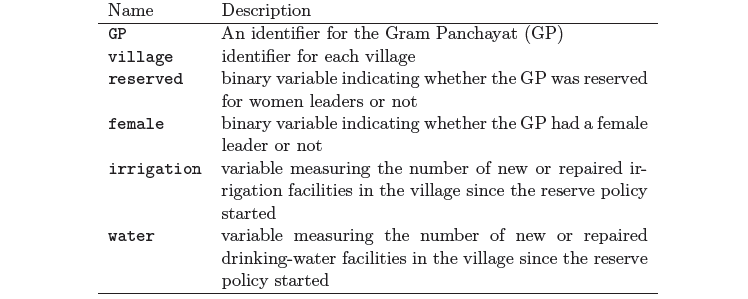
\includegraphics[width=1.1\textwidth]{women_desc.png}
\end{figure}		

\newpage
\begin{enumerate}
	\item [(a)] State a null and alternative (two-tailed) hypothesis. 
	
	\begin{itemize}
		\item Null Hypothesis : The retention policy for women among village committee leaders has no impact on the number of new or repaired drinking water facilities in the village. Mathematically speaking, this can be expressed as: where is the coefficient of the “reserved” variable in the regression model.
		\item Alternative Hypothesis: The retention policy of village committee leaders towards women has an impact on the number of new or repaired drinking water facilities in the village. Mathematically speaking, this can be expressed as: this is a double tailed substitution hypothesis, as we are testing whether the coefficients differ significantly from zero in any direction.
		
		
	\end{itemize}
	\vspace{2cm}
	\item [(b)] Run a bivariate regression to test this hypothesis in \texttt{R} (include your code!).
	\lstinputlisting[language=R, firstline=71, lastline=74]{PS02_zhuo_zhang.R} 
	\textbf{Result}:\\
   	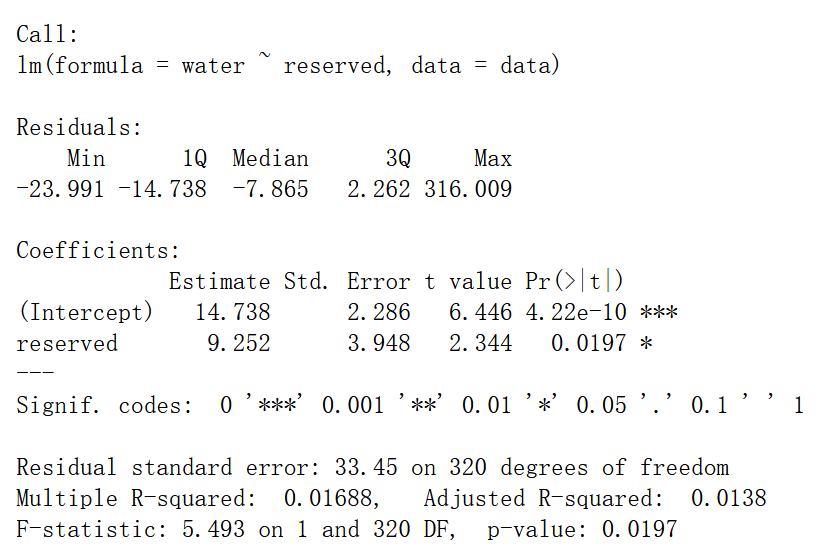
\includegraphics[width=0.8\textwidth]{01.png}
	\vspace{6cm}
	\item [(c)] Interpret the coefficient estimate for reservation policy. 
	\begin{itemize}
		\item The coefficient estimate for the ``reserved'' variable stands at 9.252, bearing a standard error of 3.948, along with an associated p-value of 0.0197. This coefficient signifies the alteration in the count of newly established or refurbished drinking water facilities within villages that correspond to a one-unit shift in the ``reserved'' variable. This variable determines whether the village council head's position is set aside for women.
		\begin{itemize}
			\item Coefficient Value: The positive coefficient estimate of 9.252 implies that, on average, when the village council head's position is reserved for women (i.e., ``reserved'' = 1), there is an approximate increment of 9.252 in the number of fresh or fixed drinking water facilities in contrast to situations with no reservation policy (i.e., ``reserved'' = 0).
	        \item Statistical Significance: The coefficient bears statistical significance, as indicated by a p-value of 0.0197, which is below the conventional significance threshold of 0.05. This suggests that the implementation of a reservation policy for women in village council head positions has a noteworthy impact on the count of new or repaired drinking water facilities in villages.
	        
	    \end{itemize}
	\end{itemize}
\end{enumerate}

\end{document}
